\subsection{Critical droplets}
\label{sec:drops}

On the sampled active side, a small active region usually disappears:
the probability of growth increases with its initial size. We placed a disordered disk of radius $R$
(sites alive with probability $1/2$) in the dead state and ran 500--1000 independent replicas per
$(q,R)$ until extinction, boundary escape, or the declared time horizon
(Fig.~\ref{fig:drop}). All replicas in the completed disordered-disk ensembles resolve
to extinction or escape. The macroscopic-growth probability $P_{\rm grow}$
rises from 0 to 1 over a factor of about 3 in $R$, and the radius at which it reaches
$1/2$ grows as $q\to\qs$: $R_c = 2.6$, 4.8, 7.9, 12.5, 21, and 42 at $q/\qs = 2.0$, 1.40,
1.20, 1.10, 1.05, and 1.02. Plotted against the inverse planar-front velocity at the same $q$,
$R_c$ is approximately linear [Fig.~\ref{fig:drop}(b)], $R_c\simeq D/v + \Delta R$ with $D = 0.207$ and an offset
$\Delta R = 1.4$ sites, consistent with relaxation of the random initial disk; equivalently,
$R_c v = 0.21$--$0.26$ over a factor of 11 in $v$. The deterministic growth
law $\ds R/\ds t = v-D/R$ has curvature radius $D/v$; the fitted initial
radius includes the offset $\Delta R$. Curvature slows a convex active
region. In this
description, linear front reversal predicts $R_c\propto1/(q-\qs)$ near
coexistence; the finite-time measurements support the relation to $1/v$ over
the sampled range. Joint resampling of the binomial droplet outcomes and
independent front runs gives a conditional 95\% interval $D\in[0.182,0.230]$;
changing the front threshold and fit start gives $D=0.199$--$0.212$.
A $2\times2$ block of live sites, the standard initial
condition of spreading experiments, is far below $R_c$: it reaches the boundary with probability
$0.042\pm0.003$ at $q = 1.4\,\qs$ and $0.20\pm0.01$ at $2\,\qs$, and with probability $0.011$ at
$1.2\,\qs$ and $0.003$ at $1.1\,\qs$ (4000 replicas each), although the active phase is the stable
one there; the $R = 0.75$ disks of Fig.~\ref{fig:drop}(a), $2\times2$ blocks in which each site is
alive with probability $1/2$, reach it with probability $0.014$ and $0.061$ at
$1.4\,\qs$ and $2\,\qs$.
Here $R_c$ is the radius at which $P_{\rm grow}=1/2$ for the specified box
and observation horizon, not a strict minimum size or an infinite-time
survival threshold. Smaller seeds have a nonzero chance to grow. The useful
nucleation diagnostic is the increase of this probabilistic radius and its
relation to the independently measured front velocity.

\begin{figure*}
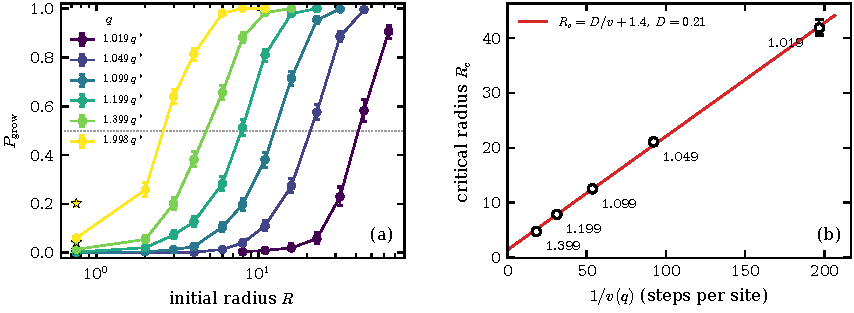
\includegraphics[width=\textwidth]{figs/fig_drop}
\caption{Critical droplets at $p = 1/2$. (a) Probability $P_{\rm grow}$ that a disordered disk of radius $R$
in the dead state reaches the lattice boundary before extinction and before
the declared time horizon, for $q/\qs$ from 1.02 to 2
(500--1000 replicas per point; at $R = 0.75$, a
$2\times2$ block with each site alive with probability $1/2$, 4000 replicas). Stars: the full
$2\times2$ block of live sites (4000 replicas). (b) Radius $R_c$ at
which $P_{\rm grow}=1/2$ against the inverse velocity of a planar front at the same $q$; labels
give $q/\qs$. The line is $R_c=D/v+\Delta R$. Disk protocols use
$L=512$--1024 and horizons $2\times10^4$--$3\times10^5$ depending on $q$;
the $2\times2$ block protocols use $L=1024$, $T=3\times10^4$.
Bars in (a) are 95\% binomial intervals from complete fixed-size replica
ensembles; vertical bars in (b) are conditional bootstrap intervals for the
interpolated $R_c$. The velocities use the corrected outer-envelope tracker.}
\label{fig:drop}
\end{figure*}

